\section{Modellering}
I denne sektion vil der blive udarbejdet matematiske modeller for alle dele af systemet. Der vil være tale om et elektronisk system (motor og feedback), der er koblet til et mekanisk system (motorakslen, rammerne og den udveksling der forbinder dem). 

\subsection{Motor}
Motoren består af en rotor med flere XXXX poler, og en stator med en permanent magnet. Den permanente magnet sørger for at feltet, der påvirker rotoren, er nogenlunde konstant - dette forsimpler udregningen af motormomentet, da det er lineært afhængigt af magnetfeltet og strømmen igennem rotorvindingerne se ligning \ref{eq:motormoment}. Motorkonstanten $K_{m}$ er afhængig af permeabiliteten i det magnetiske materiale og kan bestemmes eksperimentielt - se reference \cite{azevedo2013} XXXX.

\begin{equation}\label{eq:motormoment}
T_{m}=K_{m}i_{a}(t)
\end{equation}

Den elektroniske del af motoren kan modelleres simpelt som en modstand $R_{a}$, som beskriver den samlede modstand i vindingerne, i serie med en spole $L_{a}$, som beskriver motorens induktans. Problemet med denne model er at den ikke tager højde for den modsatrettede spænding, der genereres i motorvindingerne, når rotoren er i bevægelse. Denne spænding er lineært afhængig af rotorens omdrejningshastighed og kan modelleres som en spændingskilde i serie med modstanden og spolen se figur \ref{fig:motor_sch}. $V_{b}=K_{e}\omega(t)$, hvor $V_{b}$ er den modsatrettede spænding, $K_{e}$ er motorens elektriske konstant og $w(t)$ er omdrejningshastigheden i rad/s.

\begin{wrapfigure}[15]{r}{0.4\textwidth}
\vspace{-20pt}
	\begin{center}
	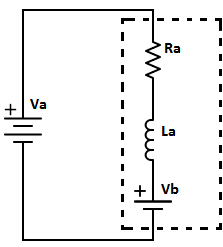
\includegraphics[scale=0.9]{Billeder/Motormodel.png}
	\end{center}
	\vspace{-10pt}
	\caption{Her ses diagrammet af den omtalte motormodel}
	\label{fig:motor_sch}
\vspace{-20pt}
\end{wrapfigure}

Ved hjælp af Kirchoff's lov om spænding kan man nu udlede en differentialligning der relaterer alle elementerne efter spændingen over dem.

\begin{equation}\label{eq:DE_motor_1}
V_{a}=i(t)R_{a}+L_{a}\dfrac{di(t)}{dt}+K_{e}\omega(t)
\end{equation}

Den mekaniske del af motoren kan beskrives som det moment der genereres og driver en belastning. Momentet for enhver roterende masse kan beskrives ved Newton's 2. lov $T_{netto}=J\alpha(t)$, hvor $J$ er intertimomentet og $\alpha$ er vinkelaccelerationen. Denne ligning kan bruges til at beskrive nettomomentet for motoren og belastningen. 

\begin{equation}\label{eq:nettomoment}
T_{netto}=T_{m}-T_{f}
\end{equation}

Ligning \ref{eq:motormoment} kunne fortælle noget om momentet fra motoren, men det er også nødvendigt at have en dæmpende effekt i form a friktion med i modellen, for at den kan svare nogenlunde til virkeligheden. Heldigvis hænger det sådan sammen at det modsatrettede moment fra friktionen kan approksimeres ret præcist til at være lineært afhængigt af akslens omdrejningshastighed - denne linearitet kan beskrives ved $T_{f}=b\omega(t)$, hvor $b$ er en friktionskonstant. Hvis man kombinerer alle tre ligninger ved at substituere dem ind i ligning \ref{eq:nettomoment}, hvor et friktionsmoment trækkes fra motormomentet, er det muligt at danne endnu en differentialligning, der afhænger af rotoren's omdrejningshastighed.

\begin{equation}\label{DE_motor_2}
J\dfrac{d\omega(t)}{dt}=K_{m}i(t)-b\omega(t)
\end{equation}

Ligning \ref{eq:DE_motor_1} og \ref{DE_motor_2} kan tilsammen beskrive motoren og dens belastning ved at relatere spændingen over motorterminalerne til omdrejningshastigheden. Det er ydermere muligt at beregne sig frem til en vinkelposition- eller acceleration ved henholdsvis at integrere eller differentiere vinkelhastigheden.

Hvis man laplace-transformerer de to ligninger kan man finde overføringsfunktionen $\dfrac{\omega(s)}{V_{a}(s)}$ ved at substituere for $I(s)$. Forholdet kan findes hvis man antager at startbetingelserne $\omega_{0}$ og $i_{0}$ er lig med nul, og at der ikke er noget \textit{disturbance moment} $T_{d}$.

\begin{equation}
G(s)=\dfrac{\omega(s)}{V_{a}(s)}=\dfrac{K_{m}}{(L_{a}s+R_{a})(Js+b)+K_{m}K_{e}}
\end{equation}

Det er muligt at forsimple systemet ved at se bort fra den elektriske del af motoren's transiente forløb. Det kan lade sig gøre fordi tidskonstanten $\frac{L_{a}}{R_{a}}$ er meget mindre end tidskonstanten for den mekaniske del $\frac{J}{b}$. I s-domænet vil det svare til at polen fra den elektriske del af motoren, befinder sig meget længere til venstre for $j\omega$-aksen end polen fra den mekaniske del. Hvis man ser bort fra den ene af polerne, kan man nu approksimere hele systemet som et 1.-ordens system, og det er en del simplere at arbejde med.

\begin{equation}
G(s)=\dfrac{\omega(s)}{V_{a}(s)}=\dfrac{K_{m}}{R_{a}(Js+b)+K_{m}K_{e}}
\end{equation}

Man har nu to muligheder for at realisere sit system: Man kan lave en \textit{White Box Model}, hvor man, gennem forsøg, finder frem til alle konstanterne i motoren og derigennem bestemmer en passende controller. Man kan også lave en \textit{Black Box Model}, hvor man måler step responsen for motorens omdrejningshastighed i forhold til spændingen over motorterminalerne. Ud fra denne respons kan man så aflæse en tidskonstant og et dc-gain, og det er alt der behøves for at kunne beskrive et 1.-ordens system.

\begin{equation}
G(s)=\dfrac{\omega(s)}{V_{a}(s)}=\dfrac{K}{\tau*s+1}
\end{equation}
